\subsection{Graph Layout}\label{subsec:graphlayout}

% Motivation for implementing algorithm ourselves
%   - alternative: use DOT language for Graphviz. 
%       - too much bloat and better understanding of algorithm if implemented manually
% Sugiyama framework
%   - 4 steps
%       - make graph acyclic
%           - mention trivial solution?
%       - assign states to layers
%       - order states in layers
%       - assign positions


% (CDE|(BC)+)|A works well in step 1 and 3, but it does not change from 2 to 3. I can use the reverse tregex in step 2: A|((BC)+|CDE)

% automaton is also missing dummy states

As mentioned in \cref{sec:related work}, the layout algorithm used in (TODO: Insert name of program) to organize and arrange the states in TAs (Timed Automaton), is called the Sugiyama framework, also known as layered graph drawing (TODO: cite sugiyama when \#343 merged). The method comprises four steps that, when combined, results in a layered graph with minimized transition crossings. These steps are discussed below, using the TA shown on \cref{fig:graph_step0}, which was constructed using the following TRE(Timed Regular Expression): $$"(CDE\mid(BC)+)\mid A"$$

% Visualise steps with different automata
\begin{center}
    \usetikzlibrary {automata,positioning}
\scalebox{0.9}{
    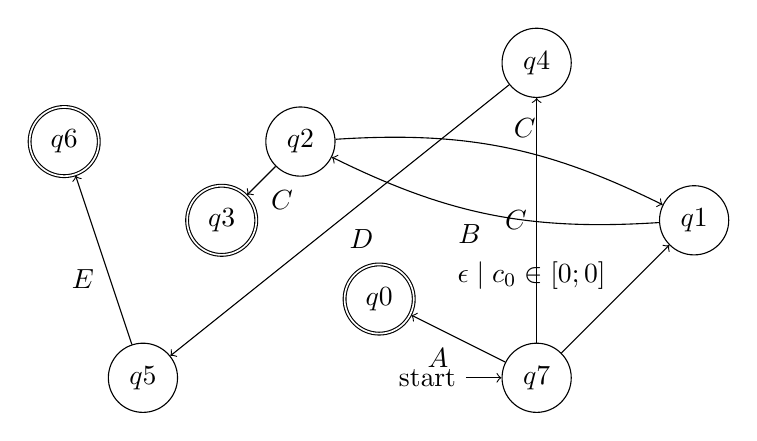
\begin{tikzpicture}[auto]
        \node[state, accepting] at (4, 1)(q0){$q0$};
        \node[state] at (8, 2)(q1){$q1$};
        \node[state] at (3, 3)(q2){$q2$};
        \node[state, accepting] at (2, 2)(q3){$q3$};
        \node[state] at (6, 4)(q4){$q4$};
        \node[state] at (1, 0)(q5){$q5$};
        \node[state, accepting] at (0, 3)(q6){$q6$};
        \node[state, initial] at (6, 0)(q7){$q7$};

        \path[->]
        (q2)edge node{$C$}(q3)
        (q1)edge [bend left=15] node{$B$}(q2)
        (q2)edge [bend left=15] node{$C$}(q1)
        (q5)edge node{$E$}(q6)
        (q4)edge node{$D$}(q5)
        (q7)edge node{$A$}(q0)
        (q7)edge node{$\epsilon\mid c_0\in[0;0]$}(q1)
        (q7)edge node{$C$}(q4)
        ;
    \end{tikzpicture}
}
\end{center}

\subsubsection{Make automata acyclic}
The first step of the Sugiyama framework is to, temporarily, make the automaton acyclic. This is necessary because subsequent steps require transitions to have a consistent direction. As described by Mazetti et al., this is done by reversing a specific list of transitions \cite{Mazetti2012}.
Mazetti describes several methods for finding this list of transitions, including using a depth first search to visit all states, and any transitions that lead to already visited states, should be reversed.
This is the method used by Graphviz' implementation of the Sugiyama framework \cite{Graphviz}. % could be irrelevant

This step, however, is trivially completed during the conversion from a TRE to a TA, since we can deduce where they are by using the semantics described by Eugene et al.
More specifically, in the construction of guaranteed iterator automata, and it's absorbed variant\cite{Eugene2001}.
In the implementation, reversible transitions are completely omitted. This is done because some reversible transitions are self-looping which do not change when reversed $(ex. q9\rightarrow q9)$, and handling all reversible transitions equally makes the algorithm much simpler. This could, however, introduce unforeseen transition crossings when reintroducing the reversible transitions, but we chose the simpler algorithm. A reversible transition can be seen on \cref{fig:graph_step1} (dashed line), described as $q2\rightarrow q1$.
% mention self loops

% insert image of step
\begin{center}
    \usetikzlibrary {automata,positioning}
\scalebox{0.9}{
    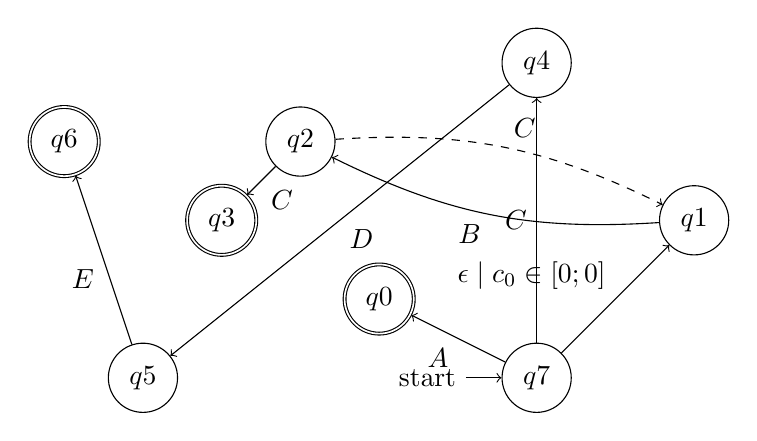
\begin{tikzpicture}[auto]
        \node[state, accepting] at (4, 1)(q0){$q0$};
        \node[state] at (8, 2)(q1){$q1$};
        \node[state] at (3, 3)(q2){$q2$};
        \node[state, accepting] at (2, 2)(q3){$q3$};
        \node[state] at (6, 4)(q4){$q4$};
        \node[state] at (1, 0)(q5){$q5$};
        \node[state, accepting] at (0, 3)(q6){$q6$};
        \node[state, initial] at (6, 0)(q7){$q7$};

        \path[->]
        (q2)edge node{$C$}(q3)
        (q1)edge [bend left=15] node{$B$}(q2)
        (q2)edge [dashed, bend left=15] node{$C$}(q1)
        (q5)edge node{$E$}(q6)
        (q4)edge node{$D$}(q5)
        (q7)edge node{$A$}(q0)
        (q7)edge node{$\epsilon\mid c_0\in[0;0]$}(q1)
        (q7)edge node{$C$}(q4)
        ;
    \end{tikzpicture}
}
\captionof{figure}{Reversible edges omitted (dashed line).}
\label{fig:graph_step1}

\end{center}

\subsubsection{Assign states to layers}
The next step is to assign states to layers. Mazetti et al. describes this process by assigning a given state to the layer index equal to the longest path from the initial state. If a transition spans multiple layers, dummy states are placed to ensure that transitions only move between adjacent layers. \cite{Mazetti2012}

This has been implemented by assigning the initial state of the automaton to layer 0, and assigning the states connected by outgoing transitions to layer 1.
This is done recursively for all outgoing states until a final state is reached.
If, at any point, a state is reached that is on the same layer or lower, it is moved to the next layer, and its outgoing states are recursively updated as well.
Dummy states are introduced if two connected states are more than one layer apart.

This implementation can be seen on \cref{fig:graph_step2}, which has resulted in a much more structured TA.

% insert image of step
\begin{center}
    \usetikzlibrary {automata,positioning}
\scalebox{0.9}{
    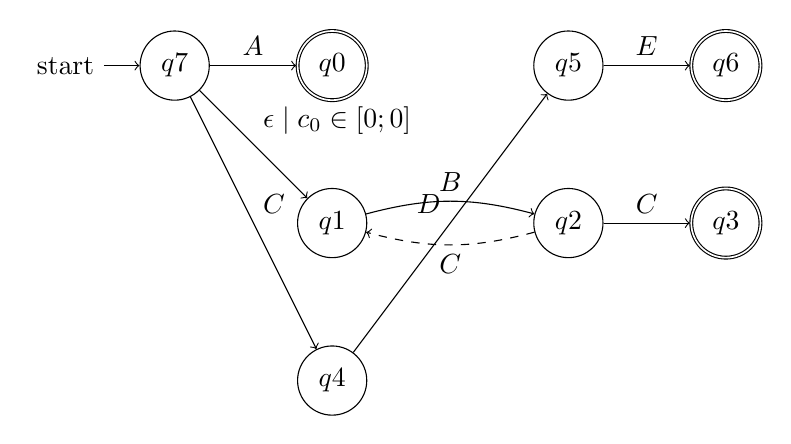
\begin{tikzpicture}[auto]
        \node[state, accepting] at (2, 0)(q0){$q0$};
        \node[state] at (2, -2)(q1){$q1$};
        \node[state] at (5, -2)(q2){$q2$};
        \node[state, accepting] at (7, -2)(q3){$q3$};
        \node[state] at (2, -4)(q4){$q4$};
        \node[state] at (5, 0)(q5){$q5$};
        \node[state, accepting] at (7, 0)(q6){$q6$};
        \node[state, initial] at (0, 0)(q7){$q7$};

        \path[->]
        (q2)edge node{$C$}(q3)
        (q1)edge [bend left=15] node{$B$}(q2)
        (q2)edge [dashed, bend left=15] node{$C$}(q1)
        (q5)edge node{$E$}(q6)
        (q4)edge node{$D$}(q5)
        (q7)edge node{$A$}(q0)
        (q7)edge node{$\epsilon\mid c_0\in[0;0]$}(q1)
        (q7)edge node{$C$}(q4)
        ;
    \end{tikzpicture}
}
\captionof{figure}{States assigned to layers.}
\label{fig:graph_step2}
\end{center}

\subsubsection{Order states in layers}
After all states have been assigned to a layer, they are ordered in those layers to ensure the smallest number of transition crossings. These crossings, more often than not, degrade the visual clarity of the automata.
Mazetti et al. formulates this by sweeping through each layer and ordering its states by the barycenter (average) of the positions of its connected states in the previous layer.
E.g. if a state is connected to two states in the previous layer, and their positions are (0, 0) and (0, 100), the given state's position would be (100, 50).
This sweep is performed thrice, once forward, once backwards, and lastly, forward again.
This ensures that both a given state's incoming and outgoing states play a role in minimizing transition crossings. \cite{Mazetti2012}

The approach implemented for this paper shares the same philosophies as the step described above, and can be seen on \cref{fig:graph_step3}.
% insert image of step
\begin{center}
    \usetikzlibrary {automata,positioning}
\scalebox{0.9}{
    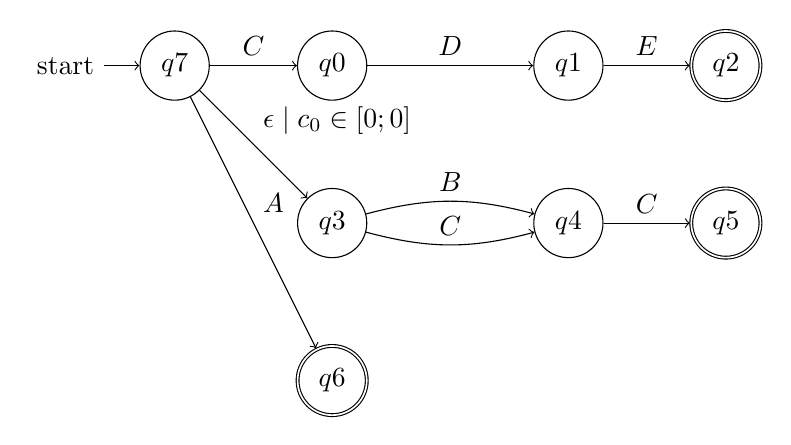
\begin{tikzpicture}[auto]
        \node[state] at (2, 0)(q0){$q0$};
        \node[state] at (5, 0)(q1){$q1$};
        \node[state, accepting] at (7, 0)(q2){$q2$};
        \node[state] at (2, -2)(q3){$q3$};
        \node[state] at (5, -2)(q4){$q4$};
        \node[state, accepting] at (7, -2)(q5){$q5$};
        \node[state, accepting] at (2, -4)(q6){$q6$};
        \node[state, initial] at (0, 0)(q7){$q7$};

        \path[->]
        (q1)edge node{$E$}(q2)
        (q0)edge node{$D$}(q1)
        (q4)edge node{$C$}(q5)
        (q3)edge [bend left=15] node{$B$}(q4)
        (q3)edge [bend right=15] node{$C$}(q4)
        (q7)edge node{$C$}(q0)
        (q7)edge node{$\epsilon\mid c_0\in[0;0]$}(q3)
        (q7)edge node{$A$}(q6)
        ;
    \end{tikzpicture}
}


\end{center}

\subsubsection{Assign positions}
The last step is to assign positions to each state. The aim of this step is to balance the graph by straightening transitions as much as possible, while minimizing the size of the graph.
Mazetti et al.'s procedure for this step is to prioritze all states in each layer based on the number of connected states in the previous layer.
More connections give a higher priority. This is quite similar to the previous step except, dummy states are given the highest prioritization.
Each state is placed based on their priority, with the ability to move states with lower priority.
Lastly, transitions between dummy states are merged, and restoring the correct transition oritentations that were reversed in the first step. \cite{Mazetti2012}

As of writing this paper, this last step of assigning the positions has not yet been implemented as in Mazetti et al. \cite{Mazetti2012}. Instead, states are simply placed based on their layer, and their index on said layer, which already offers much visual clarity. It should also be noted, that cycles are reintroduced. This is reflected in the TA on \cref{fig:graph_step4}.

% insert image of step
\begin{center}
    \usetikzlibrary {automata,positioning}
\scalebox{0.9}{
    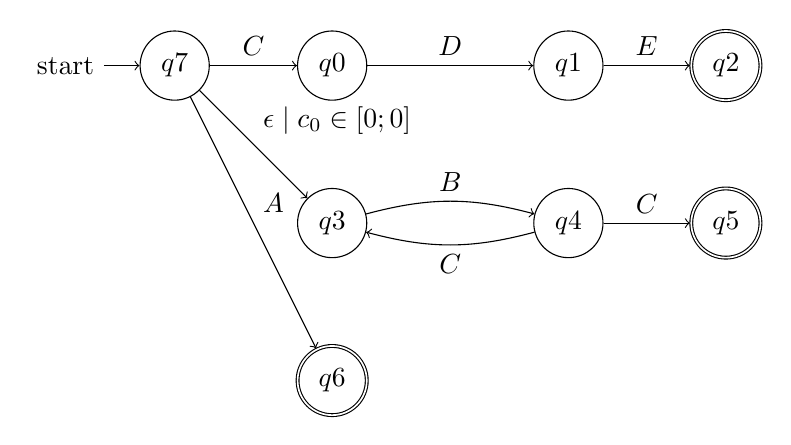
\begin{tikzpicture}[auto]
        \node[state] at (2, 0)(q0){$q0$};
        \node[state] at (5, 0)(q1){$q1$};
        \node[state, accepting] at (7, 0)(q2){$q2$};
        \node[state] at (2, -2)(q3){$q3$};
        \node[state] at (5, -2)(q4){$q4$};
        \node[state, accepting] at (7, -2)(q5){$q5$};
        \node[state, accepting] at (2, -4)(q6){$q6$};
        \node[state, initial] at (0, 0)(q7){$q7$};

        \path[->]
        (q1)edge node{$E$}(q2)
        (q0)edge node{$D$}(q1)
        (q4)edge node{$C$}(q5)
        (q3)edge [bend left=15] node{$B$}(q4)
        (q4)edge [bend left=15] node{$C$}(q3)
        (q7)edge node{$C$}(q0)
        (q7)edge node{$\epsilon\mid c_0\in[0;0]$}(q3)
        (q7)edge node{$A$}(q6)
        ;
    \end{tikzpicture}
}


\end{center}
